%!TEX root = ../dissertation.tex
\chapter{Thermal conductance via electrical noise}
\label{ch:thermal_conductance_via_electrical_noise}
A common technique in studying the various cooling pathways in a mesoscopic sample is to inject a pulse of energy into the system and monitor the time dependent electron temperature as the system returns to equilibrium. However, these ''pump-probe" experiments suffer from a few difficulties: Firstly, they yield a thermal time constant which is a convolution of the various heat capacities and thermal conductances in the problem. Secondly, the large temperature rise needed to resolve the thermal decay makes it difficult to study the linear response of low energy excitations. A steady state experiment avoids these difficulties and enables the measurement of thermal conductance in linear response at the expense of time-resolution.

In a steady state thermal experiment, a constant heating power, $\Qdot$, is injected into the electronic system and the electron temperature rise, $\Delta T$, is measured. For the experiments in this thesis, this is accomplished via Joule heating in a two terminal geometry while monitoring the change in Johnson noise temperature, $T_{JN}$ --- as discussed in chapter~\ref{section:TJN}. We can define the ratio of the applied power to the rise of Johnson noise temperature as a thermal conductance:
\begin{equation}
\Gth = \frac{\Qdot}{\Delta T_{JN}}
\end{equation}
Its important to note that $\Gth$ is not the traditional thermal conductance which describes the total heat power flowing through a material in response to a spatial temperature gradient; it is instead a generalized thermal conductance describing the heat power transferred between the electronic system and the bath under Joule heating. To extract meaningful microscopic parameters from $\Gth$ it is necessary model how the heat is entering and leaving the system as a function of these parameters. For the devices and experimental parameters presented here, the simplified thermal model shown in fig.~\ref{fig:thermal_diagram2} can be used to extract information about the electronic thermal conductivity and the electron-phonon coupling.
\begin{figure}
\centering
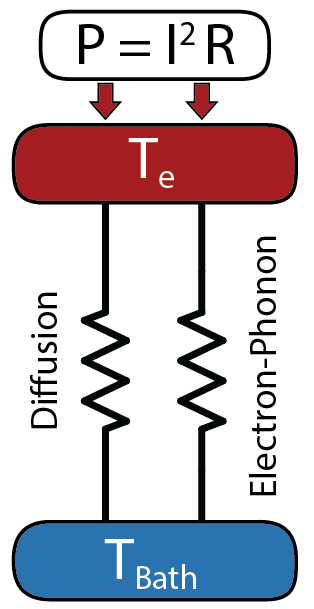
\includegraphics[width = 30mm]{figures/thermal_via_noise/thermal_diagram.png}
\caption{Simplified thermal diagram of the electronic cooling pathways in graphene relevant for the experimental conditions presented here. A current induces a heating power into the electronic system which conducts to the bath via two parallel pathways: diffusion and coupling to phonons.}
\label{fig:thermal_diagram2}
\end{figure}

\section{rectangular device}\label{section:retangularDeviceJN}
For a simple two-terminal rectangular device, the temperature measured by Johnson noise --- as given by Eqn.~\ref{eq:TJN_cont} with spatially uniform$\dot{q}$ --- is simply the spatially averaged temperature. Therefore, the total heat dissipated in linear response is then given by:
\begin{equation}\label{eq:heat_transfer}
I^2R = \Qdot = \kappa\left(\frac{W}{L}\right)\beta~\DTJN + WL~\Sigma_{e-ph}\delta T_\mathrm{b}^{\delta-1}\DTJN
\end{equation}
where $W$ and $L$ are the sample width and length, respectively, $T_\mathrm{b}$ is the bath temperature, $\kappa$ is the electronic thermal conductivity, $\Sigma_{e-ph}$ and $\delta$ are the electron-phonon parameters described in ch.~\ref{section:elph}, and $\DTJN$ is the Johnson noise temperature minus the bath temperature. The geometric factor $\beta$ depends on the shape of the electronic temperature profile which is affected by the relative strength of the two cooling terms in Eqn.~\ref{eq:heat_transfer} and must be calculated.

\subsection{Electronic conduction only}
In the absence of phonons, the temperature profile, and therefore $\beta$, can be solved analytically. For simplicity we assume that the graphene sample is homogeneous, that the approximately uniform electrical current is given by 
\begin{equation}
\mathrm{J} = -\sigma \frac{\mathrm{d}V}{\mathrm{d}x} - \alpha \frac{\mathrm{d}T}{\mathrm{d}x}
\end{equation}
and that the heat current is given by \begin{equation}
\dot{q} = -\alpha T\frac{\mathrm{d}V}{\mathrm{d}x} - \bar\kappa \frac{\mathrm{d}T}{\mathrm{d}x}
\end{equation}
where
\begin{equation}
\bar\kappa \equiv \kappa + \frac{T\alpha^2}{\sigma} = \kappa~(1+ZT).
\end{equation}
In the latter equation,  $ZT$ is the thermoelectric coefficient of merit. In the limit of negligible thermo electric effects $\bar\kappa\approx\kappa$. 

$\mathrm{d}T/\mathrm{d}x$ is the temperature gradient in the sample,  and $-\mathrm{d}V/\mathrm{d}x$ is the electric field in the sample.  $\alpha/\sigma$ is the Seebeck coefficient.  If the Joule heating is current biased, the response of graphene is dominated only by the changes in voltage $V$ and temperature $T$ to a uniform current density $\mathrm{J}$, which is applied externally, thus:
\begin{equation}\label{eq:1Dconduction_contJ}
0 = \frac{\mathrm{d}\mathrm{J}}{\mathrm{d}x}
\end{equation}
In the linear response regime, the Joule power, $\mathcal{P}$, is given by $\mathrm{J}\times E$ and thus the continuity equation for the heat current in 1D becomes:
\begin{equation}\label{eq:1Dconduction_contq}
\mathcal{P} = \frac{\mathrm{J}^2}{\sigma} =  \frac{\mathrm{d}\dot{q}}{\mathrm{d}x}
\end{equation}\label{eq:1Dconduction_diffeq}
combining the above equations we obtain \begin{equation}
\mathcal{P} = -\kappa \frac{\mathrm{d}^2 T}{\mathrm{d}x^2}
\end{equation}
assuming that $\kappa$ is approximately homogeneous throughout the sample.

The contacts serve as thermal baths and thus are held at the same temperature $T_\mathrm{b}$. Writing 
\begin{equation}
T(x) = T_\mathrm{b} + \Delta T(x)
\end{equation}
solving Eqn.~\ref{eq:1Dconduction_diffeq} using this form for the solution with the boundary conditions $\Delta T(0) = \Delta T(L) = 0$ we find a parabolic temperature profile:
\begin{equation}
\Delta T(x) = \frac{\mathcal{P}}{2\kappa}x(L-x) 
\end{equation}
The average temperature change in the sample, which is directly measured through Johnson noise thermometry, is 
\begin{equation}\label{eq:1Dconduction_Tave}
\DTJN = \DTave = \int\limits_0^L \frac{\mathrm{d}x}{L}\; \Delta T(x)  = \frac{\mathcal{P}L^2}{12\kappa}
\end{equation}
plugging in the power per unit length $\mathcal{P}$ in terms of $\sigma$ and the external voltage $V_0$,
\begin{equation}
\DTJN = \frac{V_0^2~\sigma}{12~\kappa}
\end{equation}
This non-uniform temperature profile is illustrated in Fig. \ref{fig:cartoon_Tprofile}.   
\begin{figure}
\centering
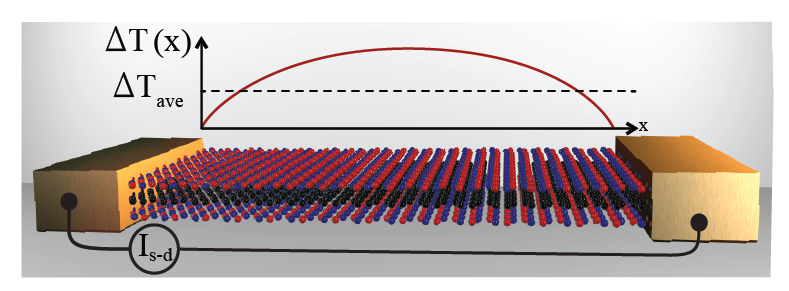
\includegraphics[width=100mm]{figures/thermal_via_noise/picture_temperature_profile.png}
\caption{Cartoon illustrating the non-uniform temperature profile within the graphene-hBN stack during Joule heating in the diffusion-limited regime.}
\label{fig:cartoon_Tprofile}
\end{figure}

Combining eqs.~\ref{eq:heat_transfer}~and~\ref{eq:1Dconduction_Tave} in the limit of no electron-phonon coupling we obtain the relation between the experimentally measured $\Gth$ and the microscopic quantity of interest $\kappa$ as
\begin{equation}\label{eq:1Dconductance_Gth}
\Gth \equiv \frac{\Qdot}{\DTJN} = \frac{12W}{L} \kappa
\end{equation}
All the information about the heating profile is contained in the factor of 12. --- i.e for a two-terminal rectangular geometry under Joule heating $\beta = 12$. If the electronic conductance follows the Wiedemann-Franz law, such that $\kappa=\sL\sigma T$, then Eqn.~\ref{eq:1Dconductance_Gth} becomes
\begin{equation}\label{eq:1Dconductance_GthWF}
\Gth = \frac{12W\sL\sigma T_\mathrm{b}}{L} = \frac{12\sL T_\mathrm{b}}{R}
\end{equation}
where R is the directly measurable, two-terminal electrical resistance.

\subsection{Phonon cooling only}
The limit of electron-phonon dominated cooling can be modeled by phonons effectively removing an isotropic amount of heat per unit area; the balance between this and Joule heating leads to a uniform temperature profile, 
\begin{equation}
\Delta T(x) = T_0 = \DTJN
\end{equation}
The heat balance equation --- Eqn.~\ref{eq:heat_transfer} with a Joule heating source --- then becomes
\begin{equation}
I^2R = WL~\Sigma_{e-ph}\delta T_\mathrm{b}^{\delta-1}\DTJN
\end{equation}
and thus the microscopic parameters governing electron-phonon coupling are related to the experimentally measured thermal conductance by
\begin{equation}
\Gth = WL~\Sigma_{e-ph}\delta T_\mathrm{b}^{\delta-1}
\end{equation}

\section{Wedge devices}
Unlike the simple rectangle where the Johnson noise temperature was simply  the mean temperature, for more complicated geometries we have to compute what effective temperature we will measure in a noise experiment given the temperature profile. An instructive example of a more complicated geometry which can also be solved analytically is a semicircular wedge as shown in fig.~\ref{fig:KCwedge}.
\begin{figure}
\centering
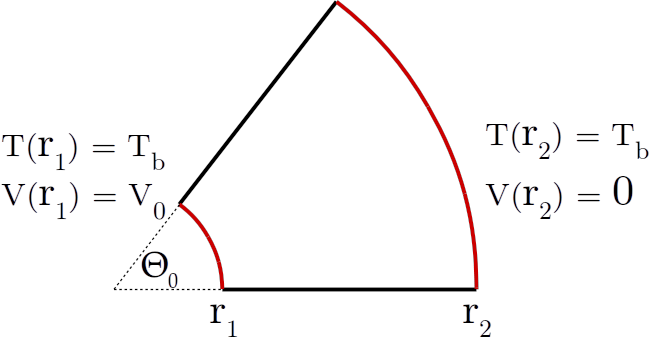
\includegraphics[width=80mm]{figures/thermal_via_noise/wedge.png}
\caption{Sketch of a wedge shaped device and boundary conditions for Joule heating. Red boundaries represent contacts where temperature is fixed at $T_\mathrm{b}$. A voltage $V_0$ is placed on the contact at $r=r_1$ while the second contact at $r=r_2$ is held at ground. Cylindrical symmetry leaves heat and charge currents independent of angle $\mathrm{\theta}$.}
\label{fig:KCwedge}
\end{figure}
The continuity equations for heat and charge current in cylindrical coordinates yield
\begin{equation}\label{eq:wedge_contJ}
\mathrm{J}(r) = -\frac{V_0\sigma}{\mathrm{ln}(r_1/r_2)}\frac{1}{r}\hat{r}
\end{equation}
and
\begin{equation}\label{eq:wedge_contq}
\frac{\mathrm{J}^2}{\sigma} = \nabla\cdot\dot{q} = \kappa\frac{\mathrm{d}^2 T}{\mathrm{d}r^2}+\frac{\kappa}{r}\frac{\mathrm{d} T}{\mathrm{d}r}
\end{equation}
Combining Eqns.~\ref{eq:wedge_contJ}~and~\ref{eq:wedge_contq} and solving using the thermal boundary conditions of fixed temperature at the contacts, the temperature profile is given by:
\begin{equation}\label{eq:wedge_Tprofile}
\Delta T(r) = \frac{V_0^2~\sigma}{2\kappa~\mathrm{ln}\left(r_1/r_2\right)^2}~\mathrm{ln}\left(\frac{r}{r_1}\right)\mathrm{ln}\left(\frac{r}{r_2}\right)
\end{equation}
The mean temperature and the Johnson noise temperature can be calculated by integrating Eqn.~\ref{eq:wedge_Tprofile} yielding,
\begin{align}
\DTave &= \int\limits_{r_1}^{r_2}T(r)~r~\mathrm{d}r \bigg/ \int\limits_{r_1}^{r_2}r~\mathrm{d}r =\frac{V_0^2~\sigma}{4~\kappa~\mathrm{ln}(r_2/r_1)}\left[\frac{r_1^1+r_2^2}{r_1^1+r_2^2}-\mathrm{ln}(r_2/r_1)\right] \\
\DTJN &= \int\limits_{r_1}^{r_2}\dot{q}(r)T(r)~r~\mathrm{d}r \bigg/ \int\limits_{r_1}^{r_2}\dot{q}(r)~r~\mathrm{d}r = \frac{V_0^2~\sigma}{12~\kappa}\label{eq:wedge_TJN}
\end{align}
The difference between the spatially averaged temperature and $\DTJN$ illustrates the power of combining Joule heating with Johnson noise thermometry --- the spatial distribution heat is injected into the system is the same as the spatial weighting function for Johnson noise measurements. Rewriting Eqn.~\ref{eq:wedge_TJN} in terms of $\Gth$ assuming the Wiedemann-Franz law we arrive at the same form as Eqn.~\ref{eq:1Dconductance_GthWF},
\begin{equation}\label{eq:wedge_GthWF}
\Gth = \frac{12\sL T_\mathrm{b}}{R}
\end{equation}
All geometric dependence is contained in the experimentally measurable two-terminal resistance $R$ and we find, similar to the rectangular geometry, $\beta = 12$.

\section{Arbitrary geometries: universality of $\beta$}
\label{section:beta}
Above we have derived two analytic examples where $\beta$ was shown to $12$. In fact, it can be shown that $\beta = 12$ is universally true in the linear response regime regardless of the geometry of the device or the form of the conductivity tensors, $\hat\sigma$ and $\hat\kappa$, provided the following conditions are met:
\begin{enumerate}
\item The device has only two electrical terminals which serve as thermal heat sinks
\item Electron cool is provided only by Wiedemann-Franz diffusion
\item $\hat\sigma$ and $\hat\kappa$ are spatially uniform
\end{enumerate}
The following derivation is adapted from a work done by Dr. Brian Skinner, MIT, altered from clarity and brevity:

Without loss of generality, we can imagine a unit voltage applied across an arbitrary two terminal device, so that the electric potential $\phi (r)$ has $\phi = 1$ at the source electrode and $\phi = 0$ at the drain. For a generic conductivity tensor $\hat\sigma$ (which may be affected by magnetic field) the electric current $\vec{\mathrm{J}}(r)$ is
\begin{equation}
\vec{\mathrm{J}}(r) = -\hat\sigma\vec\nabla\phi .
\end{equation}
Thus, the continuity equation $\vec\nabla\cdot\vec{\mathrm{J}}=0$ becomes
\begin{equation}
\vec\nabla\cdot\hat\sigma\vec\nabla\phi=0
\end{equation}
This equation, together with the boundary conditions, defines the electric potential. The boundaries at non-contact edges are assumed to be reflecting, so that $(\vec\nabla\phi)\cdot\hat{n}=0$, where $\hat{n}$ is a unit normal vector to the boundary.

The electron temperature $T(r)$, defined relative to the base temperature $T_\mathrm{b}$, obeys the heat diffusion equation
\begin{equation}
\dot{q}(r) = -\vec\nabla\cdot(\hat\kappa\vec\nabla T),
\end{equation}
if there are no extraneous sources of heat dissipation, such as electron-phonon coupling, then the steady state condition will set $\dot{q}$  equal to the dissipated Joule heating power per unit area. The Joule power is given by $\vec{\mathrm{J}}\cdot\vec{E}$, or
\begin{equation}
\dot{q}(r) = (\hat\sigma\vec\nabla\phi)\cdot(\vec\nabla\phi)
\label{eq:brian_qdot}
\end{equation}
If we assume the generalized Wiedemann-Franz relation in the linear response regime, $\hat\kappa = \hat\sigma\sL T_\mathrm{b}$, we arrive at the following relation governing the temperature:
\begin{equation}\label{eq:brian_Tdiffeq}
(\hat\sigma\vec\nabla\phi)\cdot(\vec\nabla\phi) = -\sL T_\mathrm{b}\vec\nabla\cdot(\hat\sigma\vec\nabla T).
\end{equation}
Together with the boundary conditions, this equation defines the temperature profile $T(r)$. We assume that the contacts are good heat sinks, so that $T = 0$ at both contacts,
and that no heat is lost at the boundary of the sample: $(\vec\nabla T)\cdot\hat{n}) = 0$.

Eqn.~\ref{eq:brian_Tdiffeq} makes clear that there is a close relation between the temperature profile and the electric potential. It can be shown that Eqn.~\ref{eq:brian_Tdiffeq} and the boundary condictions are satisfied by the ansatz,
\begin{equation}\label{eq:brian_Tprofile}
T(r)=\frac{1}{2~\sL~T_\mathrm{b}}\phi(r)(1-\phi(r)).
\end{equation}

From Eqn.~\ref{eq:brian_Tprofile} we can calculate the Johnson noise temperature via Eqn.~\ref{eq:TJN_cont}:
\begin{align}
\DTJN &= \int\mathrm{d}^2r\dot{q}(r)~T(r) / \Qdot \nonumber \\
&= \frac{R}{2\sL T_\mathrm{b}}\int\mathrm{d}^2r\phi(r)\left[1-\phi(r)\right]\left[\hat\sigma\vec\nabla\phi(r)\right]\cdot\left[\vec\nabla\phi(r)\right]\label{eq:brian_TJN1}
\end{align}
Here we have used $\Qdot = V^2/R = 1/R$ (assuming our voltage units). Combining Eqn.~\ref{eq:brian_Tprofile}~and~\ref{eq:brian_TJN1} we can right $\DTJN$ is terms of only the temperature profile:
\begin{align}
&= \sL T_\mathrm{b}R\int\mathrm{d}^2rT(r)\vec\nabla\cdot(\hat\sigma\vec\nabla T) \nonumber \\
&= \sL T_\mathrm{b}R\int\mathrm{d}^2r(\vec\nabla T(r))\cdot(\hat\sigma\vec\nabla T(r)).\label{eq:brian_TJN2}
\end{align}
Eqn.~\ref{eq:brian_TJN2} was found using integration by parts, and noting that either $T$ or $\vec\nabla T$ vanishes at the boundaries of the sample.

The geometric factor $\beta$ is defined by
\begin{equation}
\frac{1}{\beta}\equiv\frac{\DTJN~\sL~T_\mathrm{b}}{\Qdot~R}.
\end{equation}
Plugging in Eqn.~\ref{eq:brian_TJN1}
\begin{equation}
\frac{1}{\beta} = \frac{1}{2~\Qdot}\int\mathrm{d}^2r\phi(1-\phi)(\hat\sigma\vec\nabla\phi)\cdot(\vec\nabla\phi).
\label{eq:brian_midDer1}
\end{equation}
On the other hand, inserting Eqn.~\ref{eq:brian_Tprofile} into eqn.~\ref{eq:brian_TJN2} and rearranging gives
\begin{align}
\frac{1}{\beta} &= \frac{1}{4~\Qdot}\int\mathrm{d}^2r\left[\vec\nabla(\phi(1-\phi))\right]\cdot\left[\hat\sigma\vec\nabla(\phi(1-\phi))\right] \nonumber \\
&=\frac{1}{4~\Qdot}\int\mathrm{d}^2r(1-2\phi)^2(\vec\nabla\phi)\cdot(\hat\sigma\vec\nabla\phi) \nonumber \\
&=\frac{1}{4~\Qdot}\left[\int\mathrm{d}^2r(\vec\nabla\phi)\cdot(\hat\sigma\vec\nabla\phi) - \int\mathrm{d}^2r~4\phi(1-\phi)(\vec\nabla\phi)\cdot(\hat\sigma\vec\nabla\phi)\right].\label{eq:brian_midDer2}
\end{align}
The second term in Eqn.~\ref{eq:brian_midDer2} is identical to the right hand side of Eqn.~\ref{eq:brian_midDer1} multiplied by 2, and it is therefore equal to $2/\beta$. Thus:
\begin{align}
\frac{1}{\beta} &= \frac{1}{4~\Qdot}\int\mathrm{d}^2r(\vec\nabla\phi)\cdot(\hat\sigma\vec\nabla\phi) \nonumber \\
&=\frac{1}{12~\Qdot}\int\mathrm{d}^2r(\vec\nabla\phi)\cdot(\hat\sigma\vec\nabla\phi) \nonumber \\
&=\frac{1}{12~\Qdot}\int\mathrm{d}^2r~\dot{q}(r)\label{eq:brian_midDer3}
\end{align}
The final step in Eqn.~\ref{eq:brian_midDer3} comes from realizing the integrand is simply the Joule heating power given in eqn.~\ref{eq:brian_qdot}, and thus
\begin{equation}
\beta = 12
\end{equation}

\section{Experimental setup}
\begin{figure}[b]
\centering
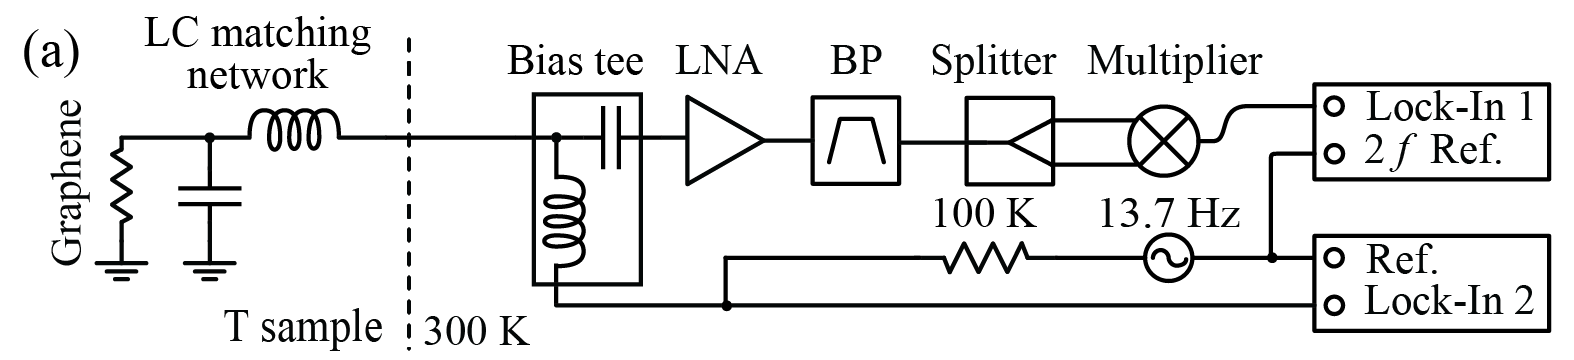
\includegraphics[width=130mm]{figures/thermal_via_noise/Schematic_Joule_heating.png}
\caption{Simplified schematic of thermal conductance measurement setup. A low frequency Joule heating current is pass through the sample using a lock-in amplifier and and corresponding temperature is measured using Johnson noise thermometry. The noise signal is measured as the second harmonic of the heating current as $\Delta T \sim I^2$}
\label{fig:schematic_Joule_heating}
\end{figure}
To sensitively measure $\DTJN$, the autocorrelation Johnson noise thermometry circuit described in chapter~\ref{ch:johnson_noise_thermometry} can be modified to allow a DC current to Joule heat the sample. Fig.~\ref{fig:schematic_Joule_heating} show a simplified schematic of a thermal conductance measurement setup. A low frequency $(f{\sim 13}~Hz)$ current is generated by a lock-in amplifier\footnote{This lock-in is also used to measure the two-terminal resistance $R$} at frequency $\omega = 2\pi~f$ and passed through the sample\footnote{It is because of this need to pass a DC current through the matching network and into the sample that the LC tanks used are setup in a low-pass configuration} using a bias tee. If the current is given by:
\begin{equation}
I(t) = I_0\sin(\omega t)
\end{equation}
the total heating power dissipated in the device is
\begin{equation}
\Qdot(t) = I_0^2R\sin^2(\omega t)
\end{equation}
and the corresponding temperature rise in Johnson noise temperature is 
\begin{align}
\DTJN(t) &= \frac{I_0R}{\Gth}\sin^2(\omega~t) \nonumber \\
&=\frac{I_0R}{2~\Gth}\left(1-\cos(2\omega~t)\right)
\end{align}
The $2\omega$ component of the corresponding noise signal is then measured by a second lock-in synced to the second harmonic of the Joule heating current (phase shifted by $\pi/2$) as shown in Fig.~\ref{fig:schematic_Joule_heating}.

\begin{figure}
\centering
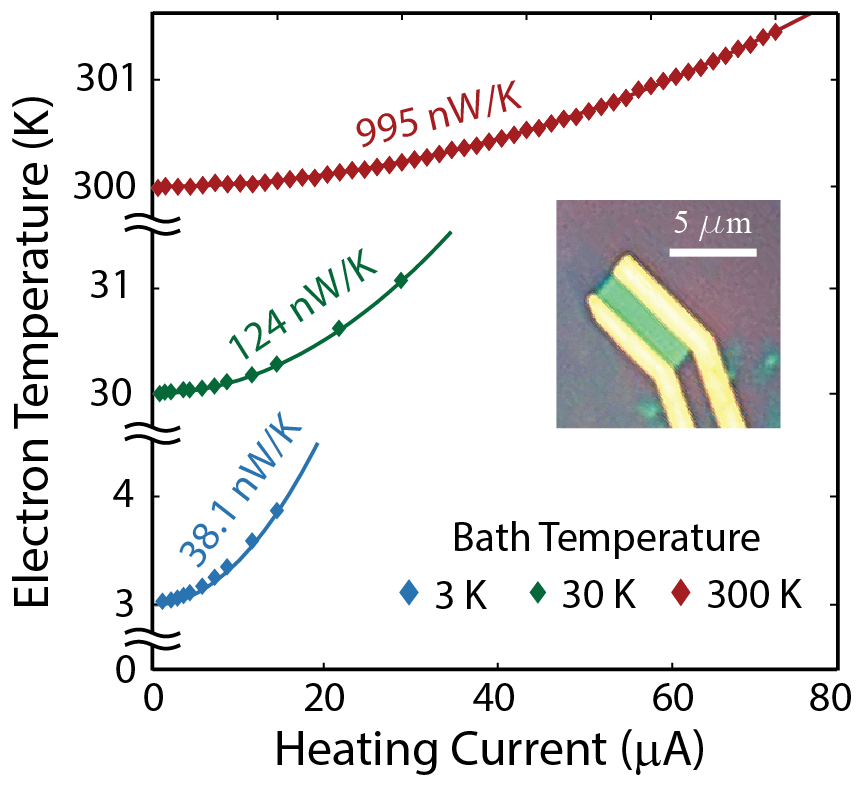
\includegraphics[width=60mm]{figures/thermal_via_noise/quadratic_Joule_heating.png}
\caption{Electron temperature of a two-terminal graphene device (inset) as a function of a Joule heating current for three different bath temperatures. The temperatures follow an $I^2$ heating law with the curvature determined by the generalized thermal conductance $\Gth$ which increases with the bath temperature. Here electron temperature is defined as the Johnson noise temperature as discussed in section~\ref{section:retangularDeviceJN}}
\label{fig:quadratic_Joule_heating}
\end{figure}
Fig.~\ref{fig:quadratic_Joule_heating} shows how the electronic temperature mesoscopic device responds to a heating current. As expected for the linear response regime, the temperature rise follows an $I^2$ heating curve with curvature governed by the generalized thermal conductance. The thermal conductivity, $\kappa$, can be extracted in the low temperature regime using the factor $\beta = 12$ derived in section~\ref{section:retangularDeviceJN} --- a example of which is shown in comparison to the Wiedemann-Franz law in Fig.~\ref{fig:examplekappa}. At low temperature the assumptions required to show $\beta = 12$ are met and the measured thermal conductivity follows the Wiedemann-Franz law. At high temperature phonons spoil assumption $2$ in section~\ref{section:beta} and $\kappa$ can no longer be accurately extracted from $\Gth$.
\begin{SCfigure}
\centering
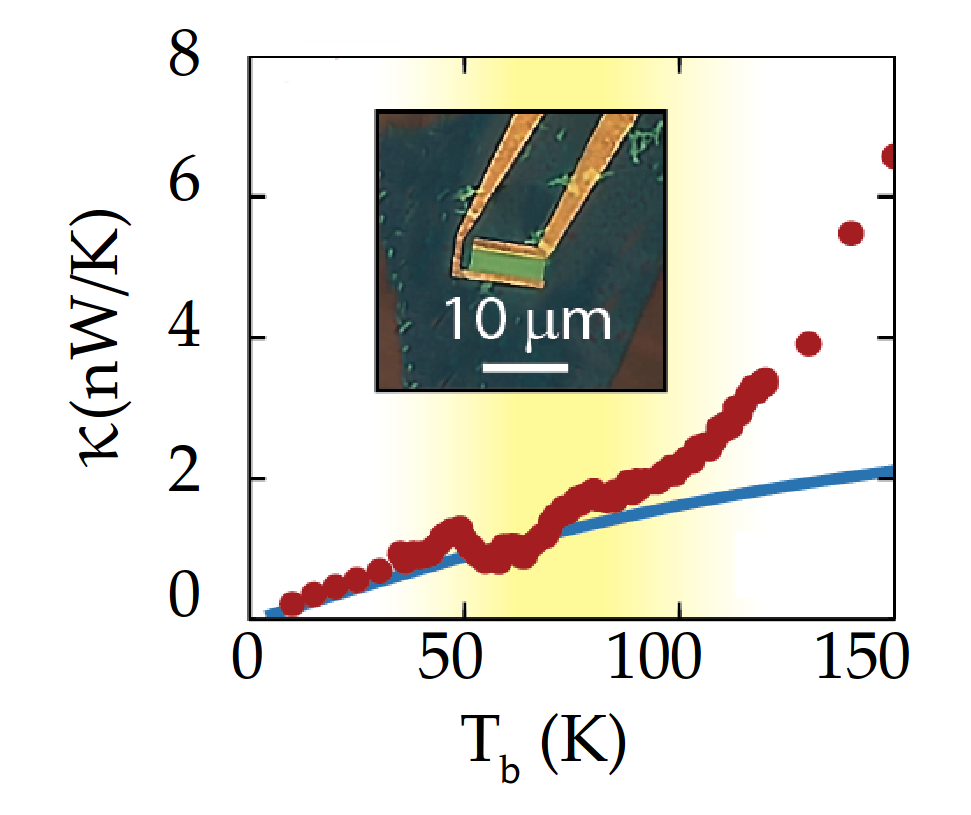
\includegraphics[width=50mm]{figures/thermal_via_noise/kappa.png}
\caption{Thermal conductivity extracted from $\Gth$ measured using the circuit shown in Fig.~\ref{fig:schematic_Joule_heating} assuming $\beta = 12$. At low temperature $\kappa$ can accurately be extracted from $\Gth$ and the measured thermal conductivity follows the Wiedemann-Franz law (solid blue line). At higher temperatures phonons spoil the assumptions needed for $\beta = 12$ and prevent the accurate measurement of $\kappa$}
\label{fig:examplekappa}
\end{SCfigure}